\chapter{Background}

\section{Embedded Databases}
\subsection{DuckDB}
DuckDB is an in-memory, embedded, columnar, OLAP Database\cite{DuckDBPaper} developed as a successor to MonetDBLite\cite{MonetDBLitePaper} in the embedable database OLAP niche.
\begin{center}
    \begin{tabular}{l p{.8\textwidth}}
        \textbf{Embedable}         & The database is a single file with no dependencies, and is easily embeddable in and usable from applications written in Python, R, Java, Julia, Swift and Rust\cite{DuckDBDocs}. \\
        \textbf{Cost-Aware}        & In addition to common rule-based optimisations, DuckDB uses a cost-model and statistics collected at runtime for its logical optimizer.                                          \\
        \textbf{Extensible}        & DuckDB supports loadable WASM extensions.                                                                                                                                        \\
        \textbf{Language Agnostic} & DuckDB communicates through the C-ABI and uses its heap, as a result it cannot take advantage of language/compiler specifics (e.g. data representation).                         \\
        \textbf{Columnar}          & To better support OLAP access patterns. This hurts OLTP performance, which is better suited to a nary storage, furthermore the only supported indexes are zonemaps/min-max
        indexes and adaptive radix trees. Neither offer lookup performance comparable to hash indecies, or indexed arenas as demonstrated in \ref{sec:intro_experimentation}.                                         \\
        \textbf{Concurrency}       & DuckDB uses a combination of optimistic and multiversion concurrency control.                                                                                                    \\
    \end{tabular}
\end{center}
\noindent
\subsubsection{System Design}
The authors describe the design as \textit{"textbook"}\cite{DuckDBPaper}.
\begin{center}
    \includegraphics[scale=1]{_drawio/background/images/duckdb_system.pdf}
\end{center}
\subsubsection{Vector Volcano Processing}
DuckDB uses a \textit{vector volcano} processing model. The interpreter takes a dynamically constructed tree of operators, wherein each operator pulls data from input operators on demand much like with volano processing.
However instead of pulling individual tuples, \mintinline{Cpp}{DataChunks} are passed, each containing a tuple of column vectors for a row-range of the previous operator's output.
\begin{center}
    \includegraphics[scale=1]{_drawio/background/images/duckdb_operators.pdf}
\end{center}


\subsection{SQLite}
SQlite is a lightweight embedded database\cite{SQLitePaper}, and is currently the most deployed database in the world\cite{SQLiteWebsite}.
Unlike DuckDB it is designed for OLTP workloads, and as such stores rows in an nary record format.
\subsubsection{System Design}
\begin{center}
    \includegraphics[scale=1]{_drawio/background/images/sqlite_system.pdf}
\end{center}
\subsubsection{Virtual Database Engine Bytecode}
One of the key elements of SQLite's design is that rather than using traditional physical plan (i.e. trees of operators) it instead uses a simple bytecode, interpreted on the virtual database engine.
\begin{minted}{SQL}
CREATE TABLE users (
    id INTEGER PRIMARY KEY AUTOINCREMENT,
    name VARCHAR NOT NULL,
    premium BOOLEAN NOT NULL,
    credits MEDIUMINT NOT NULL,
    CONSTRAINT premcredits CHECK (premium OR credits >= 0)
);

-- Get Total Premium credits
EXPLAIN SELECT SUM(credits) FROM users WHERE premium = TRUE;
\end{minted}
When run with SQLite (compiled with \mintinline{bash}{-DSQLITE_ENABLE_EXPLAIN_COMMENTS}) the following bytecde is returned:
\begin{center}
    \begin{tabular}{l l | l l l l l | l}
                      &                 & \multicolumn{5}{c|}{\textbf{Registers}} &                                                                                                               \\
        \textbf{addr} & \textbf{opcode} & \textbf{p1}                             & \textbf{p2} & \textbf{p3} & \textbf{p4}     & \textbf{p5} & \textbf{comment}                                  \\
        \hline
        0             & Init            & 0                                       & 13          & 0           & null            & 0           & \mintinline{bash}{Start at 13        }            \\
        1             & Null            & 0                                       & 1           & 2           & null            & 0           & \mintinline{bash}{r[1..2]=NULL       }            \\
        2             & OpenRead        & 0                                       & 5           & 0           & 4               & 0           & \mintinline{bash}{root=3 iDb=0; users}            \\
        3             & Rewind          & 0                                       & 9           & 0           & null            & 0           & \mintinline{bash}{               }                \\
        4             & \qquad Column   & \qquad  0                               & \qquad 2    & \qquad 3    & \qquad null     & \qquad 0    & \qquad \mintinline{bash}{r[3]= cursor 0 column 2} \\
        5             & \qquad Ne       & \qquad  4                               & \qquad 8    & \qquad 3    & \qquad BINARY-8 & \qquad 83   & \qquad \mintinline{bash}{if r[3]!=r[4] goto 8   } \\
        6             & \qquad Column   & \qquad  0                               & \qquad 3    & \qquad 3    & \qquad null     & \qquad 0    & \qquad \mintinline{bash}{r[3]= cursor 0 column 3} \\
        7             & \qquad AggStep  & \qquad  0                               & \qquad 3    & \qquad 2    & \qquad sum(1)   & \qquad 1    & \qquad \mintinline{bash}{ accum=r[2] step(r[3]) } \\
        8             & Next            & 0                                       & 4           & 0           & null            & 1           & \mintinline{bash}{              }                 \\
        9             & AggFinal        & 2                                       & 1           & 0           & sum(1)          & 0           & \mintinline{bash}{accum=r[2] N=1    }             \\
        10            & Copy            & 2                                       & 5           & 0           & null            & 0           & \mintinline{bash}{r[5]=r[2]         }             \\
        11            & ResultRow       & 5                                       & 1           & 0           & null            & 0           & \mintinline{bash}{output=r[5]       }             \\
        12            & Halt            & 0                                       & 0           & 0           & null            & 0           & \mintinline{bash}{                  }             \\
        13            & Transaction     & 0                                       & 0           & 3           & 0               & 1           & \mintinline{bash}{usesStmtJournal=0 }             \\
        14            & Integer         & 1                                       & 4           & 0           & null            & 0           & \mintinline{bash}{r[4]=1            }             \\
        15            & Goto            & 0                                       & 1           & 0           & null            & 0           & \mintinline{bash}{              }                 \\
    \end{tabular}
\end{center}

\subsubsection{JIT Compilation for SQLite}
In order to improve performance, without burdening developers with the additional development \& maintenance
cost of writing a JIT compiler, one can be generated from the interpreter. This strategy has been attempted with SQLite\cite{SQLiteJITCompiler} and advertised a $1.72\times$ speedup over a seelction of TPC-H queries.

\section{Code Generation for Databases}
\subsection{Holistic Integrated Query Engine}
The Holistic Integrated Query Engine\cite{HIQUEPaper} is a single-threaded, JIT code generating, general purpose relational database that implements queries using a C++ code generator and attached C++ compiler.
Typical just-in-time compilation powered databases use a lower-level representation, and pass this to a bundled compiler (e.g. LLVM), however there are several advantages to using C++ as the target representation.
\begin{center}
    \begin{tabular}{l p{.8\textwidth}}
        \textbf{Visibility}   & The output is easily inspectable C++, and the compiler can optionally include debug information, or additional instrumentation when compiling queries to assist in debugging the engine, and the compiler itself verifies the type safety of code. While HIQUE was evaluated using GCC, it is possible to swap out the compiler for another (e.g. Clang) for additional features without difficulty. \\
        \textbf{Templates}    & The templates used by the code generator are also written in C++, making them easier to write and maintain.                                                                                                                                                                                                                                                                                          \\
        \textbf{Optimisation} & A broad range of optimisations (including for the native hardware) can be performed, and the compiler has access to the entire context of the query code.
    \end{tabular}
\end{center}
The significant downside to source generation is the time \& system resource taken by using a full C++ compiler, which increases with query complexity, and the level op optimisation. This is particularly problematic for small queries associated with OLTP workloads.
\\
\\ The main focus of HIQUE is to avoid the poor instruction and data cache performance associated with the volcano processing model by using hand-optimised templates to generate cache concious code for common operations. A large focus of this to improve the performance of iteration over rows.
By using the known types of fixed-length tuples, and accessing through direct referencing \& pointer arithmetic, no function calls are required to tuple access, and the system can use the size of the tuple to avoid random accesses to block sizes only resident in the lower levels of the memory hierarchy.
\\
\\ HIQUE also uses a Partitioned Attributed Across (PAX) record layout\cite{PAXStorageModel} that stores fixed size ranges of rows as a tuples of column vectors, this provides the row lookup advantages of nary stprage (all items of a given row are stored in the same page, requiring at most of page load for access), as well as the better cache performance of columnar storage (allowing simple linear scans over columns). This is conceptually similar to the \mintinline{Cpp}{DataChunks} abstraction used by DuckDB.
\subsubsection{System Design}
\begin{center}
    \includegraphics[scale=1]{_drawio/background/images/HIQUE_system.pdf}
\end{center}
\subsubsection{Relevance to emdb}
The cost of using a full C++ compiler at compile time is the only major downside to the many upsides of generating high-level code.
\\
\\ By lifting query compilation to the application's compile time, the same benefits can be achieved with emdb, without needing to do any query compilation work at runtime.
\\
\\ The only performance downside of this is that chip-specific parameters (e.g. cache sizes) are only available when the binary is run, if it compiled for an architecture in general, rather than for the exact chip of the machine the application will run on.

\section{Incremental View Maintenance}

\begin{tcbraster}[raster columns=2,raster equal height]
    \begin{definitionbox}{Views}
        \centerline{\textbf{Recompute on Access}}
        \begin{minted}{SQL}
CREATE VIEW my_view AS SELECT * FROM ..;            
        \end{minted}
        An alias for a query, typically a \mintinline{SQL}{SELECT} statement, that can be queried like a table. The view's query is used each time it is accessed.\cite{Postgres16Docs}
    \end{definitionbox}
    \begin{definitionbox}{Materialized Views}
        \centerline{\textbf{Recompute on Change}}
        Views with results cached. The contained query is only recomputed after a change in the data the query relies on. Beneficial for expensive queries that are frequently accessed and depend on infrequently changing data.
    \end{definitionbox}
\end{tcbraster}
\noindent
The aim of incremental view maintenance is to support views on data that \textbf{Never Recompute} in their entirety, but instead can updated \textit{incrementally} using changes applied to source relations.
\begin{center}
    \includegraphics[scale=1]{_drawio/background/images/ivm.pdf}
\end{center}
The cost reduction from recomputing operators to recomputing the deltas of operators can also be applied recursively.

\subsection{DBToaster}
DBToaster is an incremental view maintenance code generation tool, that generates C++, Spark (including a distributed spark target) and OCaml implementations from queries.
\subsubsection{SQL Support}
A SQL syntax is supported (with incomplete compliance with ASNI SQL-92) to construct select queries
on streams\cite{DBToasterSQLReference} of tuple changes and are the only way to write/mutate relations in the system.
Tables are supported, but are static and cannot be modified after load.
\\
\\ By forgoing complex write insert, update and delete queries, DBToaster avoids much of the complexity in combining
transactions, constraints and delta queries (the calculus used for generating delta queries has no support for
relation mutation).
\\
\\ A restricted set of conditionals \& functions are supported, and external functions are possible (depending on backend used).

\subsubsection{System Design}
\begin{center}
    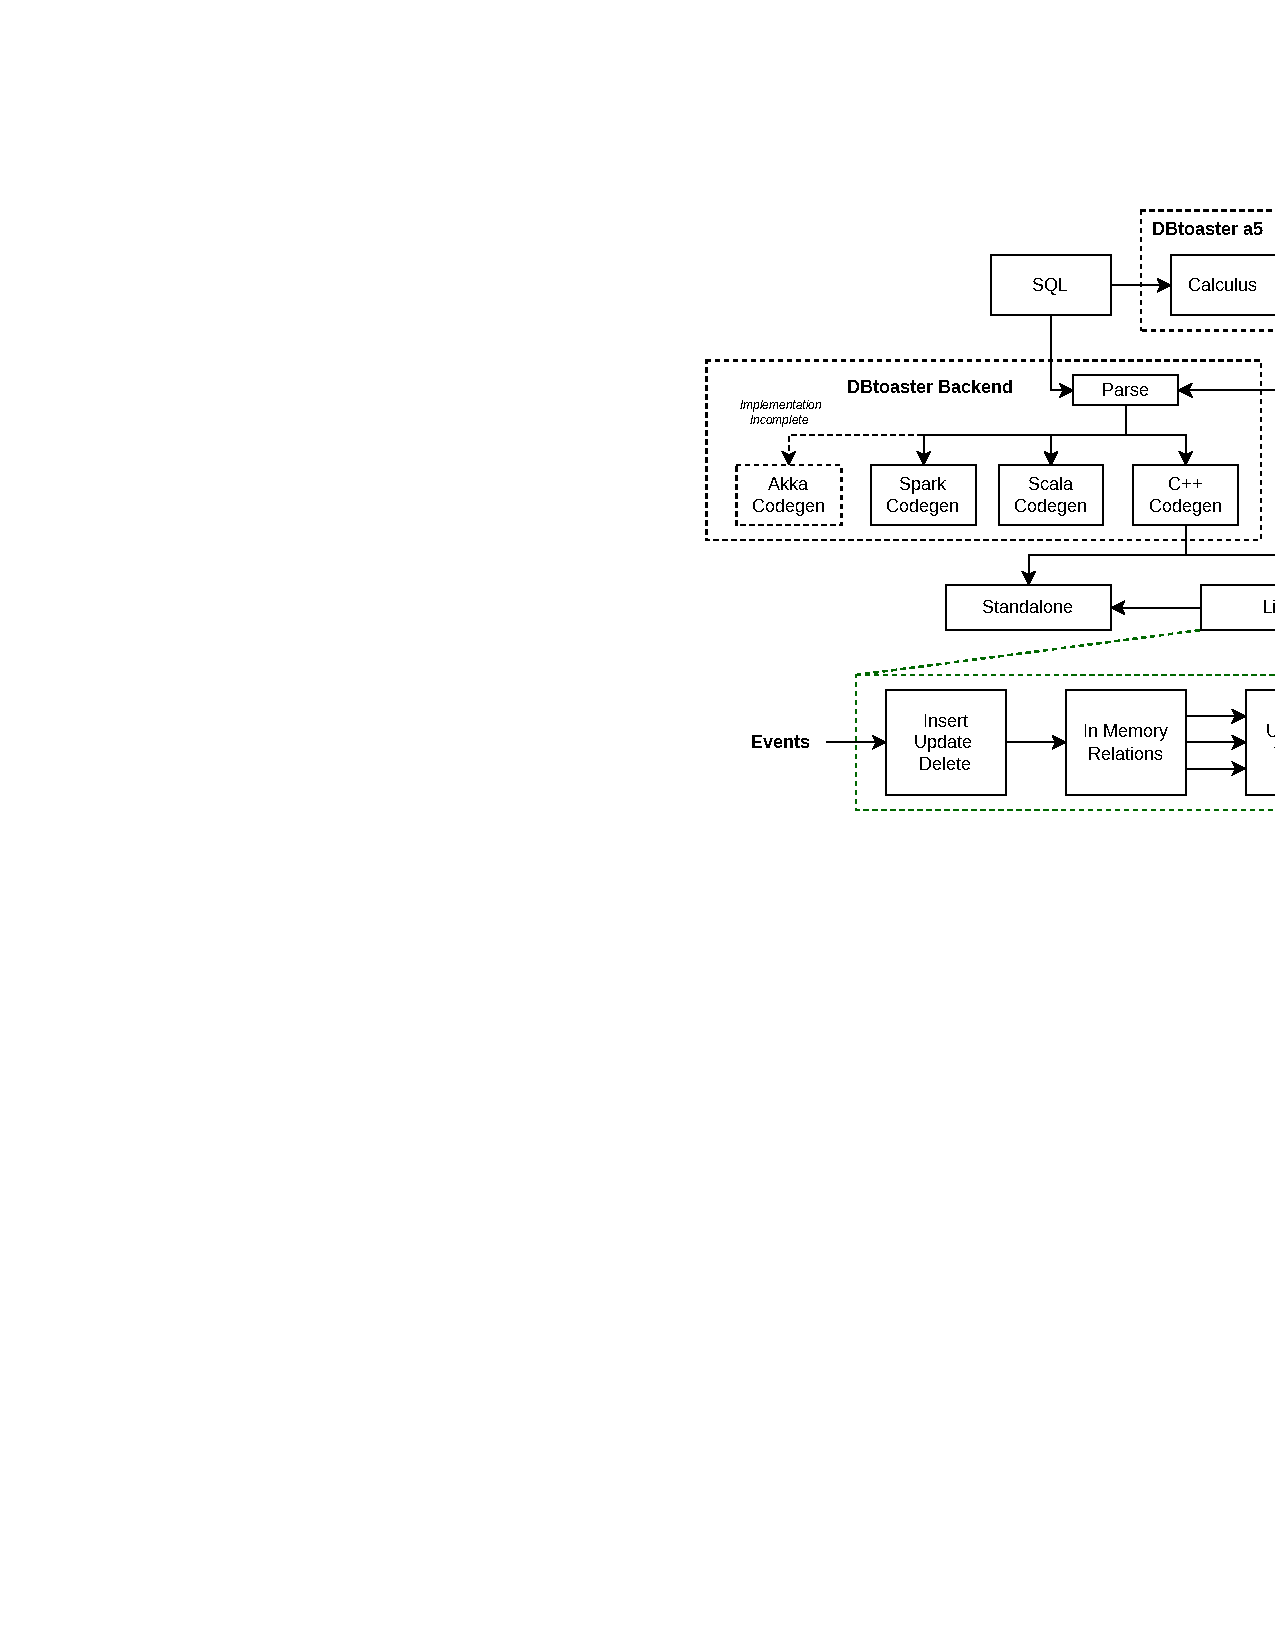
\includegraphics[scale=1]{_drawio/background/images/dbtoaster_system.pdf}
\end{center}
One of the key advantages for DToaster is that the code generated is easily embeddable in applications, which provides the same advantages as discussed in \ref{sec:intro_experimentation}.

\subsubsection{Aggregation Calculus}
DBToaster lifts queries parsed from SQL and represented by a simplified relational algebra into its own aggregation calculus (AGCA). AGCA represents data through generalized multiset relations (GMRs) which are mappings from the set of tuples to the multiplicites of those tuples in relations.
\begin{center}
    \includegraphics[scale=1]{_drawio/background/images/dbtoaster_agca_syntax.pdf}
\end{center}
\begin{center}
    \includegraphics[scale=1]{_drawio/background/images/dbtoaster_agca_eval_gmrs.pdf}
\end{center}
Evaluation rules for the language are provided in the paper \textit{DBToaster: Higher-order Delta Processing for Dynamic, Frequently Fresh Views}\cite{DBToasterHigherOrderDeltaProcessing} and are ommitted for brevity.
\\
\\ SQL translation is done by converting to relational algebra (with bag semantics), upon which operations can be reduced to union ($+$) and join ($\bowtie$) by judicial allowance for infinite relations. For example $\sigma_{A<B}(R)$ is rewritten as $R \bowtie (A < B)$ despite $A < B$ being an infinitely large set of possible tuples.
\begin{minted}{SQL}
                    SELECT * FROM R WHERE B < (SELECT SUM (D) FROM S WHERE A > C);
\end{minted}
\[Sum_{[A,B]}(R(A,B) \ast (z := Sum_{[]}(S(C<D) \ast (A > C) \ast D)) \ast (B < z))\]
From AGCA the delta queries can be generated by simple recursive descent of the AGCA expression, applying the following rules:
\[
    \begin{split}
        \Delta(Q_1 + Q_2) & \equiv (\Delta Q_1) + (\Delta Q_2) \\
        \Delta(Q_1 \ast Q_2) & \equiv ((\Delta Q_2) \ast Q_2) + (Q_1 \ast (\Delta Q_2)) + ((\Delta Q_1) \ast (\Delta Q_2)) \\
        \Delta (x := Q) & \equiv (x := (Q + \Delta Q)) - (x := Q) \\
        \Delta (-Q) & \equiv - (\Delta Q) \\
        \Delta(Sum_{\overrightarrow{A}}Q) & \equiv Sum_{\overrightarrow{A}}(\Delta Q) \\
        \Delta ( x \ \theta \ 0) \equiv \Delta x \equiv \Delta c & \equiv 0 \\
    \end{split}
\]
As AGCA is closed under taking the delta query, this process can be reapplied for higher order delta queries to incrementally compute delta queries.
\section{Embedded Domain Specific Languages}
Embedded Domain Specific Languages (eDSLs) allow for the expression of domain specific logic and
concepts within a host (typically general purpose) programming language. Such eDSLs are typically
distributed as a library and implemented using features of the host language, not requiring
additional compilation steps by external tools.
\\
\\ eDSLs can be roughly categorised as the following:
\begin{center}
    \begin{longtable}{p{.1\textwidth} p{.8\textwidth}}
        \textbf{String\newline Based} & {
                The most popular implementation, wherein a library is provided to process strings of the
                eDSL at runtime. By using strings, any syntax is possible at the cost of language integration.
                \newline
                \newline This lack of integration prevents the eDSL from being compiled at application compile time,
                introducing a runtime performance cost as well as correctness as generic bugs such as type
                errors (in the eDSL) can exist even after the application is successfully compiled.
                The lack of integration also prevents automatic support by the host language's tools
                (e.g. language server).
                \newline
                \newline Typically stringified DSLs also dont allow for the host language to be embedded/used
                inside the DSL, as no compiler is available at runtime to compile embeddings, and the wider
                context of the program is erased at application compile time.
                \newline
                \newline This is the approach taken by most SQL client libraries.
        }                                 \\
        \\
        \textbf{Compiler Provided}    & {
                Full compiler integration can be supported by implementing the eDSL within the host language's compiler.
                \newline
                \newline This allows for custom syntax, eDSL compilation \& analysis to occur at the same time
                as the host language, and full integration with the host language's tools.
                As the eDSL code exists in the host's compiler, the eDSL compiler can also use context and
                analysis from outside the eDSL to aide in analysis (e.g. type inference for SQL queries based
                on the types of variables their output are assigned to).
                \newline
                \newline This comes at significant development \& decision cost (as do all changes to
                major compilers).
                \newline
                \newline Some common examples include the embedding of JSX expressions in javascript.
                \begin{minted}{javascript}
// ... some program logic
const element = <h1>Hello, {world_formatter(name)}</h1>; 
            \end{minted}
                Or the SQL syntax for Langiage Integrated Queries (LINQ) in C\#.
                \begin{minted}{cs}
int[] data = [ ... ];
var evenData = from num in data where (num % 2) == 0 select num;
foreach (var num in evenData) { Console.WriteLine(num); }
            \end{minted}
        }                                 \\
        \\
        \textbf{Host\newline Native}  & {
                Rather than creating new syntax, the language is instead implemented using only constructs
                from the host language. Often this takes the form of libraries providing rich typed APIs,
                and exist on a vague spectrum from eDSL, to simply a library with a complex API.
                \newline
                \newline The eDSL design is restricted by the host language, and this strategy is more
                often employed in languages that allow custom operators and evaluations contexts (monads \& effects).
                \newline
                \newline For example Gigaparsec\cite{GigaparsecRepo} is a Haskell parser combinator library implemented with a DSL.
                \begin{minted}{haskell}
-- Parse a hell[l]*o world and return the world
parser :: Parser String
parser = (atomic (string "he")) >> (manyN 2 (atomic (string "l"))) 
      >> (atomic (string "o ")) >> (atomic (string "world"))

parse @String parser "hellllllllllllo world"
                \end{minted}
            }
        \\
        \\
        \textbf{Macro Based}          & {
        The eDSL is implemented as a macro taking inputs provided by the host compiler in a syntax agnostic form (e.g. text, or tokens).
        This allows for custom syntax, while also allowing the eDSL to be compiled at application compile time without requiring changes to the host compiler.
        \newline
        \newline For example the Racket language is designed specifically for developing eDSLs through macros.
        \newline
        \newline One of the most popular languages to support this feature is Rust, which supports procedural macros, where a user defined macro can run
        arbitrary rust code at compile time, taking compiler tokens and producing new tokens and compiler diagnostics.
        \newline
        \newline For example the yew\cite{YewRepo} web frontend framework for rust contains a JSX-like \mintinline{rust}{html! { .. }} macro that
        takes in html, with embedded rust (in place of javascript).
        \begin{minted}{rust}
let user = ... ;
let page = html! {
    <div class="container">
        <h1>{ "Hello World!" }</h1>
        <p>{ 
            if let Some(name) == user {
                format!("And hello {}!", name)
            } else {
                "And hello stranger!".to_owned()
            }
            }</p>
    </div>
};
                \end{minted}
        Another example is sqlx\cite{sqlxRepo}, which is a SQL toolkit for rust that can validate \& type check query strings against a development database, at application compile time.
        \begin{minted}{rust}
// this query string is not a string, but rather a string tokn to be parsed & 
//used by sqlx at compile time
let countries = sqlx::query!(
        "
-- Get the number of premium users in each credit bracket, given a minimum
-- number of credits
SELECT name, COUNT(*) as count
FROM users
GROUP BY (credits / 100) * 100
WHERE premium AND credits > ?
        ",
        min_credits
    )
    .fetch_all(&connection_pool)
    .await?;
                \end{minted}
        }                                 \\
    \end{longtable}
\end{center}
\noindent
One of the key strengths of the non-string based eDSL implementations are the ability to embed the host language in the eDSL.
This limits the requirement for the user to consider an entirely different language (syntax, semantics \& libraries), or to
manage complex conversions where the eDSL and host language interface.
\begin{quote}
    \textit{The problem is simple: two languages are more than twice as difficult to use as one language.
        The host and query languages often use different notations for the same thing, and convenient
        abstractions such as higher-order functions and nesting may not be available in the query language.
        Interfacing between the two adds to the mental burden on the programmer and leads to complex code,
        bugs, and security holes\dots}
    \\ \textbf{- A Practical Theory of Language-Integrated Query}\cite{PracticalTheoryLINQPaper}
\end{quote}

\subsection{Rust Procedural Macros}
Rust supports several types of macros as part of its procedural macro system. Unlike C/C++ macros are invoked and run after tokenisation.
\\ \begin{longtable}{l p{.8\textwidth}}
    \textbf{Declarative} & {
            Using \mintinline{rust}{macro_rules!} to declare a set
            of patterns and substitutions.
            \begin{minted}{rust}
macro_rules! log_assign {
    ($variable:ident = $value:expr) {
        let $variable = $value;
        println!("trace: {} = {}", stringify!($variable), $value)
    };
}
log_assign!(x = 5);
        \end{minted}
    }                                                                                                                                                                                                  \\                                                                                                                                                                                                 \\
    \textbf{Attribute}   & {
            Applied to modules, structs, enums, or functions. They can take their
            own arguments, and the tokenstream representing the structure they are tagged to.
            \newline
            \newline For example the divan benchmarking library uses an attribute macro to declare parameters for benchmarks.
            \begin{minted}{rust}
#[divan::bench(
    name = "random_inserts",
    types = [Foresight, Naive, DuckDB, SQLite],
    consts = TABLE_SIZES
)]
fn inserts<'a, T, const N: usize>(bencher: Bencher) { ... }
        \end{minted}
    }                                                                                                                                                                                                  \\
    \\
    \textbf{Derive}      & {
    Macros used to derive a named trait for a struct or enum. Standardised to allow for their invocation by the \mintinline{rust}{#[derive(..)]} attribute macro.
    \begin{minted}{rust}
#[derive(Clone, Debug, PartialEq, Eq, Hash)]
struct Foo {
    name: String,
    premium: bool,
    credits: i32,
}
        \end{minted}
    }                                                                                                                                                                                                  \\
    \textbf{Functional}  & { Macros that can be invoked like functions, and take arbitrary tokens as input. Examples include \mintinline{rust}{vec![..]} and \mintinline{rust}{println!(" ... ", ..)}.
    }                                                                                                                                                                                                  \\
\end{longtable}
\noindent
All of these macros (including \mintinline{rust}{macro_rules!}) are implemented by procedural macros which are compiled and executed as follows:
\begin{center}
    \includegraphics[scale=1]{_drawio/background/images/rust_proc_macro.pdf}
\end{center}
A simple functional macro can be declared defined as follows:
\begin{minted}{rust}
use proc_macro::TokenStream;
extern crate proc_macro;

#[proc_macro]
fn my_macro(tk: TokenStream) -> TokenStream {  /* Can emit compiler diagnostics from here */}
\end{minted}
\begin{center}
    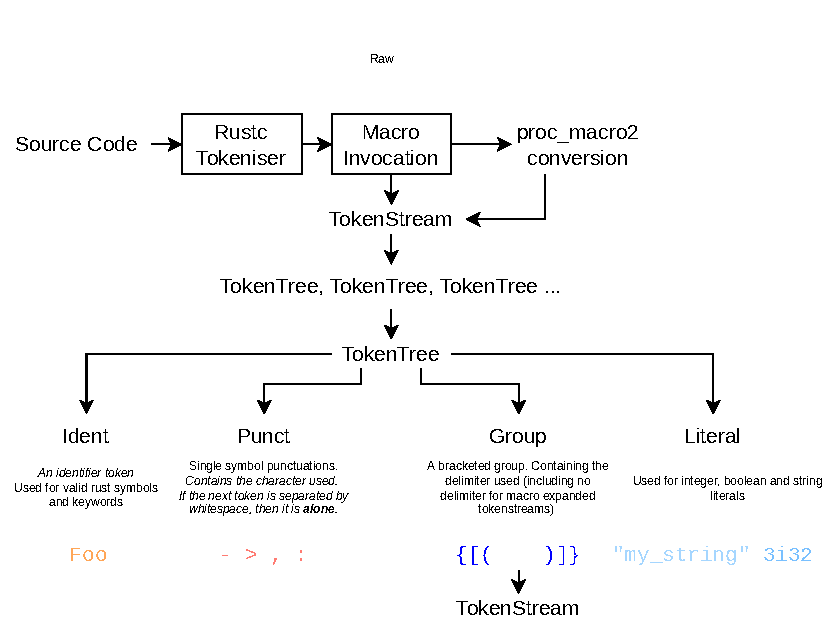
\includegraphics[scale=1]{_drawio/background/images/tokenstreams.pdf}
\end{center}
In order to generate output tokens we can either construct outselves, or use the quasi-quoting library \mintinline{rust}{quote!} to construct tokenstreams from rust snippets.
\begin{minted}{rust}
let row_type = ... ;
let filter_fn_code = quote!{
    fn filter(row: #row_type) -> Option<#row_type> {
        // wrap the user's code with a function to constraint its types. Any incorrect user 
        // code's errors will be propagated back to the original positions in the source as 
        // the spans for user_filter are from the source.
        fn do(#row_fields) -> bool { #user_filter }

        if do(#get_row_fields) { None } else { Some(row) }
    }
}
\end{minted}
